\section{Introduction}
The continuous growth in the number of objets (active satellites and space debris) has significantly raised the probability of collisions, endangering the safety of spacecrafts and satellite constellations. Hence, in order to ensure the safety and organization of activities in space, it has become crutial to quickly develop and enhance Space Situational Awareness (\textit{SSA}).


\begin{figure}[ht]
    \centering
    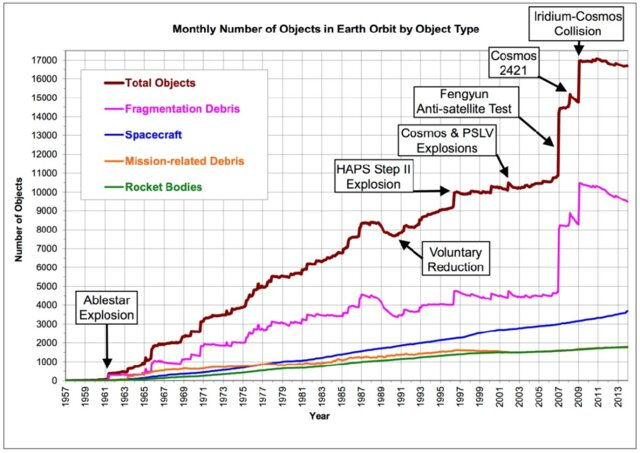
\includegraphics[width=0.8\columnwidth]{Figures/Growth-of-orbital-space-object-including-space-debris-NASA-Orbital-Debris-program_W640.jpg}
    \caption{Timeline of orbital space debris growth.}
    \label{fig:orbital_debris_growth}
\end{figure}

In this context, \textit{SSA}, which is defined as the knowledge and characterization of space objects and their operational environment, has evolved into a pivotal solution  to mitigate the growing hazards in space. While terrestrial \textit{SSA} has worked as the foundational framework, the dynamic evolution of the space environment needs a paradigm shift towards space-centric \textit{SSA}. This strategic transition entails considerable advantages in precision, operational efficiency, and system stability as compared to its terrestrial counterpart.


The area under surveillance now extends from low Earth orbits (LEO) to a terrestrial radius of at least 100,000 km. This broader coverage essentially includes all objects in orbit, encompassing both artificial and natural entities that may pose potential risks. However, there is a remarkable interest in the Low Earth Orbits due to the increasing density of satellite deployments and space activities within this region.

With the objective of  reaching the desired scope of monitoring, the adoption of advanced remote sensing and continuous monitoring technologies  has been proved essential. These technologies enable the precise identification and analysis of space threats, including debris and asteroids, contributing to a strong and proactive \textit{SSA}.


In this context, there is an imperative need for the development of specialized simulators tailored to the precise detection and tracking of space debris. These simulators must be able to provide a faithful representation of the space environment, allowing  the training and validation of \textit{SSA} strategies to work.


Space Situational Awareness, particularly in the realm of debris detection and tracking, stands as a critical component for space safety and sustainability. The adoption of advanced technologies, the transition to space-based \textit{SSA}, and the development of specialized simulators are essential steps toward the effective management of risks in orbit.

In conclusion, the increasing challenges arising from the growing number of objects in space underscore the need for a comprehensive approach to Space Situational Awareness (SSA). To address this issue, the integration of advanced technologies and the development of specialized simulators become pivotal elements. These measures collectively play a crucial role in ensuring the safety and sustainability of activities within Earth's orbit. By combining cutting-edge technologies with purpose-built simulators, we can effectively navigate the evolving complexities associated with managing risks in space.


\subsection{Motivación para Mejorar el Simulador de \textit{SSA}}

Recognizing the urgent need to systematically register and locate space debris, an initial version of a Space Situational Awareness (SSA) simulator was developed. This simulator, characterized by a basic design and a notably disorganized code structure (explained in Section \ref{s: Code}), is being requested for improvement to achieve preliminary results.

The main motivation for enhancing the SSA simulator comes from the necessity to integrate a specialized photometry module. Photometry, which involves precise measurements of light emitted by celestial entities, is of utmost importance for the detailed characterization of space debris. The addition of this module is expected to enable a more accurate simulation of the visual attributes of celestial objects in space, thereby strengthening the simulator's capacity to faithfully replicate real-world conditions.

In the process of integrating the new photometry module, the primary objective is to determine the effective range of the sensors. This step is pivotal as it serves as the foundation for the development of essential positioning functions. By accurately establishing the sensor range, these functions will facilitate the strategic positioning of observers in specific orbits. The goal is to ensure optimal visibility of the target by a minimum of 1 observer. This meticulous approach not only enhances the simulator's spatial accuracy but also improves its ability to replicate real-world observational scenarios with greater precision.

Moreover, when considering the evaluation of simulator accuracy, the focus extends beyond a general assessment based on observer numbers and average visibility times. The intention is to delve into the intricate interplay between these factors, seeking to identify patterns and dependencies that may impact the simulator's predictive capabilities. Through an analysis of how the simulator responds to variations in observer counts and average visibility times, valuable insights into the subtleties of its performance under diverse conditions can be obtained. This comprehensive examination is indispensable for validating the simulator's effectiveness in providing reliable space situational awareness, thereby establishing a robust foundation for advancements in the understanding and monitoring of space debris.


